\documentclass[12pt]{article}
\usepackage[utf8]{inputenc}
\usepackage{graphicx}
\usepackage{amsmath}
\usepackage{amsfonts}
\usepackage{amssymb}
\usepackage{subcaption}
\usepackage{float}
\usepackage{tikz}
\usepackage{listings}
\usepackage{color}
\usepackage{parskip}
\usepackage{hyperref}
\usepackage{mathrsfs}


\hypersetup{
    colorlinks=true,
    linkcolor=black,
    citecolor=black,
    filecolor=black,
    urlcolor=black
}
\usepackage[left=1in,right=1in,top=1in,bottom=1in]{geometry}
\captionsetup{justification=centering}

\title{Theoretical \& Mathematical Deep Dive: RMMs \& Derivatives}
\author{Alyssa Brittany Chen}
\date{Apr. 10, 2023}

\begin{document}

\maketitle


\tableofcontents

\newpage

\section{Introduction}
Automated Market Makers (AMMs) such as Uniswap and PancakeSwap are decentralized exchanges (DEX) that utilize an algorithmic trading rule that determines how two assets are to be exchanged through two users. These AMM-based DEXs operate primarily through liquidity pools, where liquidity providers (LP) deposit assets into the pool and are rewarded with a fraction of the fees generated on the AMM, usually distributed as LP tokens. This practice of depositing assets to earn rewards is known as yield farming. 

\subsection{Automated Market Makers \& Liquidity}
As traders buy and sell assets on AMMs, insufficient liquidity can lead to high-borrow lending spreads, which can lead to capital efficiency and impermanent loss. (explain why this is bad) 

AMM exchanges are usually based on a constant function– Bancor was one of the first AMM-based DEXs to implement the constant product market maker (CPMM), which is based off the constant product function: x*y=k. This formula accounts the range of prices for two tokens according to the available quantities (liquidity) of each token. When the supply of token X increases, the token supply of Y must decrease, and vice-versa, to maintain the constant product K. 
\begin{figure}[H]
    \centering
    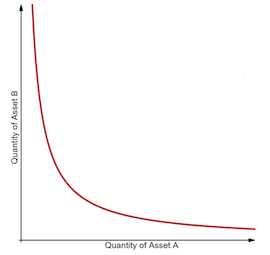
\includegraphics[width=0.5\linewidth]{constant_product.png}
    \caption{Constant Product Function}
    \label{fig:constant_product}
\end{figure}

On the other hand, constant sum market makers (CSMM) follow the formula x+y=k. However, this formula allows arbitrageurs to drain one of the reserves if the off-chain reference price between the tokens is not 1:1, which is why AMMs rarely follow the CSMM model. 
\begin{figure}[H]
    \centering
    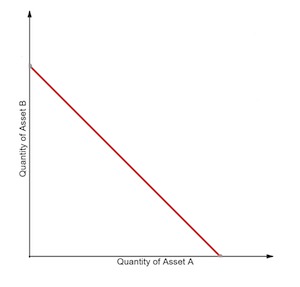
\includegraphics[width=0.5\linewidth]{constant_sum.png}
    \caption{Constant Sum Function}
    \label{fig:constant_sum}
\end{figure}

The final market maker we will cover in this article is the constant mean market maker (CMMM), which enables the creation of AMMs that can have more than two tokens and be weighted outside of the standard 50/50 distribution. For a liquidity pool with three assets, the equation would be the following:
\[
(x*y*z)^{\frac{1}{3}}=k
\]
where the weighted geometric mean of each reserve remains constant (i.e. \href{https://balancer.fi/}{Balancer}).

\section{Limitations of AMMs}
\subsection{Impermanent Loss \& Capital Inefficiency}
Impermanent loss (also known as 'negative gamma' in finance) and low capital inefficiency are two limits of AMMs that affect both liquidity providers and traders.

Consider the following example of impermanent loss: After an LP deposits assets into a pool, the price of one of the deposited assets changes significantly compared to the value when initially deposited. As a result, the ratio of assets in the pool will also fluctuate due to arbitrage trading and rebalancing prices that occur with external markets– therefore, in some cases depositing assets could lessen the LP’s positional value, which is the essence of impermanent loss. In other words, this loss is “impermanent” because the loss is recoverable if prices return to its original state when liquidity was initially deposited. On the other hand, the impermanent loss becomes permanent if the LP decides to withdraw their liquidity from the pool at this new price ratio.

Capital inefficiency refers to how effectively liquidity (capital) within a pool is used to facilitate trades without leading to large price impacts. Low capital efficiency indicates that large amounts of liquidity are required to facilitate trades without moving the market price significantly. An ideal DeFi protocol is able to optimally utilize deposited assets to ensure a balanced and efficient market– high spreads is an indication of inefficiency. As a result platforms with high spreads may result in loss of market share over time in comparison to other platforms offering more favorable rates, and this can be unfavorable for LPs because their capital isn't utilized as effectively, leading to lower returns. An example of calculating impermanent loss can be found in ~\ref{subsec:impermanent}.\

Replicating Maker Markets allow users to directly control their impermanent loss by defining a target price around which liquidity will be most concentrated. In the context of traditional markets, this is similar to setting a price in a limit order where a trader specifies the price at which they're willing to buy or sell an asset. RMMs seek to address these limitations via algorithmic strategies to better replicate the ideal liquidity curves and trading functionalities of traditional order book markets, allowing for more efficiency, flexibility, and risk management control.

\section{RMMs Explained}
\subsection{Portfolios \& Continuous Rebalancing}
Simply put, an RMM is an AMM whose portfolio value matches a target payoff. Now, let’s investigate the case of an Uniswap LP, whose value is determined by its underlying assets and their performance over time. When the value of one asset with respect to the other asset changes, the portfolio must be rebalanced such that the composition of value is equally 50-50 in each asset. This rebalancing occurs by arbitrageurs who put one asset in and take another asset out, in order to maintain the pool composition to equal 50-50 value. When the rebalancing occurs, whoever made the trade will have paid a trading fee. This trading fee is earned by all the liquidity providers of the pool. Therefore, as more trades (rebalancing) occurs, their portfolio value will grow over time (the specific fees are determined by the protocol of the specific AMM protocol).

In a Replicating Market Maker, the portfolio is always being rebalanced in a way that it matches a desired payoff. In RMMs, the goal is to replicate or mimic the payoff of certain financial instruments or desired outcome. Unlike traditional AMMs which rely on a predefined mathematical formula to set prices and manage liquidity, RMMs actively manage their portfolios to ensure that the outcome of trading within these markets closely follows a predetermined financial model or payoff structure.

RMMs use algorithms as a mechanism to continuously adjust the composition of their liquidity pools in order to ensure that the value of the pool aligns with the desired payoff structure over time. This process involves algorithmically trading assets within the pool or with external markets to maintain the target allocation and payoff outcome.

\subsection{Replicating Portfolios}

A replicating portfolio (also known as a hedge) is defined as a portfolio of assets that exhibit the same properties as the asset being referenced. In this context, there can be state and dynamic replications. State replication alludes to the portfolio sharing the same cash flows as the reference asset with a stagnant change state, while dynamic replication indicates that the portfolio has a differing cash flow than the reference asset,  but shares the same Greeks (meaning for infinitesimally small changes to underlying market parameters, the asset and portfolio price are altered in the same way). Due to the behaviors of the asset and portfolio’s partial derivatives at a singular point, dynamic replication must occur frequently. 

Replicating portfolios provide a framework for assessing and managing risk-- they do so by allowing traders to replicate the payoff structures of complex financial instruments. This concept also has important implications within DeFi, where derivatives are increasingly used to hedge risk, manage exposure, and facilitate liquidity provision in a permissionless and decentralized manner. 
\section{Derivatives}
Why do we use derivatives? The answer is actually quite simple-- derivatives are used as a tool to analyze or speculate on an assets price in the future without having to purchase that asset itself. For example, if a user believed Tesla's stock would rise in the near future, the user is would then purchase the right to buy shares to Tesla's stock in the future for a set price.

A derivative is defined as a financial contract that derives its values from its underlying assets, i.e. shares, securities, commodities, etc. Derivatives that are bought and sold privately (over-the-counter) are not regulated, and derivatives in exchanges are bought and sold via regulated systematic contracts.
There are three main types of derivatives: futures \& forwards, options, and swaps. This paper will mainly focus on options and futures in the next few sections.
\subsection{Call Options}
A call option in traditional financial markets is a contract between a buyer and seller that gives the right to purchase an asset for a predetermined (strike) price up until an expiration date. This allows the buyer to purchase the stock by exercising the call– however, the buyer does not have the obligation to do so. On the other hand, the seller shorting (selling) the call option has the obligation to sell the asset at the strike price. 

In DeFi, these call options are collateralized to simulate the legally enforceable nature of asset delivery via one part to the other. A covered call occurs when collateral is deposited and the call option is sold. 

In long calls, buyers have the option to openly purchase shares. Purchasing a long call at strike price gives buyers the option to plan ahead. For example, if a tech company frequently has new product launches at around the same time each year, the company’s stock price has the ability to appreciate after the launch. 

Short Calls indicate an open obligation to sell shares. Until the expiration date, the seller is obligated to sell shares of the stock at strike price. Short calls are generally used to increase and boost income. 

Investors in long call options hope for the underlying stock price to rise above the exercise price, and on the contrary, short call investors want the underlying stock price to stay below the exercise price. 

\subsection{Greeks \& Black Scholes}\label{subsec:greeks}
In DeFi, the concept of Greeks—borrowed from traditional finance (TradFi)—plays a crucial role in analyzing the sensitivity of various derivative instruments and protocols to different market factors. While the Greeks are primarily used in options trading, their interpretation in DeFi can extend to protocols with automated market makers and liquidity provision mechanisms.

\textbf{Delta (\(\Delta\))}: In DeFi, Delta measures the sensitivity of an asset's price to changes in the price of the underlying token. For instance, in an automated market maker (AMM), Delta can represent how the liquidity pool's token ratio shifts in response to price changes of one of the assets in the pool.

\textbf{Gamma (\(\Gamma\))}: Gamma refers to the rate of change of Delta in response to changes in the price of the underlying asset. In DeFi protocols, Gamma may be important for strategies like yield farming or liquidity mining, where changes in the ratio of tokens due to price movements can impact potential returns.

\textbf{Vega (\(V\))}: Vega represents sensitivity to volatility in both TradFi and DeFi. In decentralized options or derivative markets, Vega can quantify how a liquidity provider’s position might gain or lose value based on increased volatility in the price of the underlying assets.

\textbf{Theta (\(\Theta\))}: In DeFi options or time-dependent strategies, Theta measures the sensitivity of the position's value to the passage of time. For example, in protocols that lock liquidity for a set duration, Theta reflects the decay in value as the lock-up period approaches expiration.

\textbf{Rho (\(\rho\))}: Rho measures sensitivity to interest rates. While interest rate sensitivity is more commonly observed in TradFi, DeFi protocols that involve borrowing or lending, such as Aave or Compound, might see Rho influencing the value of liquidity positions due to changes in lending or borrowing rates.

Black Scholes, Black-Scholes-Merton or BSM refers to the differential equation used by traders to price options contracts, and requires five main inputs:
\begin{enumerate}
    \item The underlying stock's price
    \item Option's strike price
    \item Time to option's expiry
    \item Stock's volatility
    \item Risk free interest rate
\end{enumerate}

Formula:
\begin{align*}
    C = SN(d_1) -Ke^{rt}N(d_2),
\end{align*}
where $d_1 = \frac{ln_{s}^{k} + (r+ \sigma_{v}^{2})t}{\sigma_s \sqrt{t}}$ and $d_2=d_1-\sigma_s \sqrt{t}$.
\begin{enumerate}
    \item $S$-The current or underlying stock's price
    \item $C$- Call option's price
    \item $K$- Strike price
    \item $r$- Risk free interest rate
    \item $t$- Time to option's maturity
    \item $N$- Normal distribution
\end{enumerate}
\subsection{Forwards \& Futures}
Imagine you are a baker, famous for your apple pies, but apple prices fluctuate drastically between 10-40 cents/lb depending on the harvest season. In order to hedge against market volatility, you and the apple farmer set up a contract to apples at 15 cents/lb, regardless of the market price. This is an example of a forward contract. 

On the other hand, futures are a legal contract to buy or sell a commodity asset or security at a set price at a specified date in the future. These contracts are standardized on futures exchanges. The seller of the contract has an obligation to deliver that asset at the expiration date, while the buyer takes on the obligation to buy and receive the asset at expiry date.

There are two main forwards and futures curves, which are attributed to prices over time, and is used to determine whether the contract price is rising of falling:
\begin{figure}[H]
    \centering
    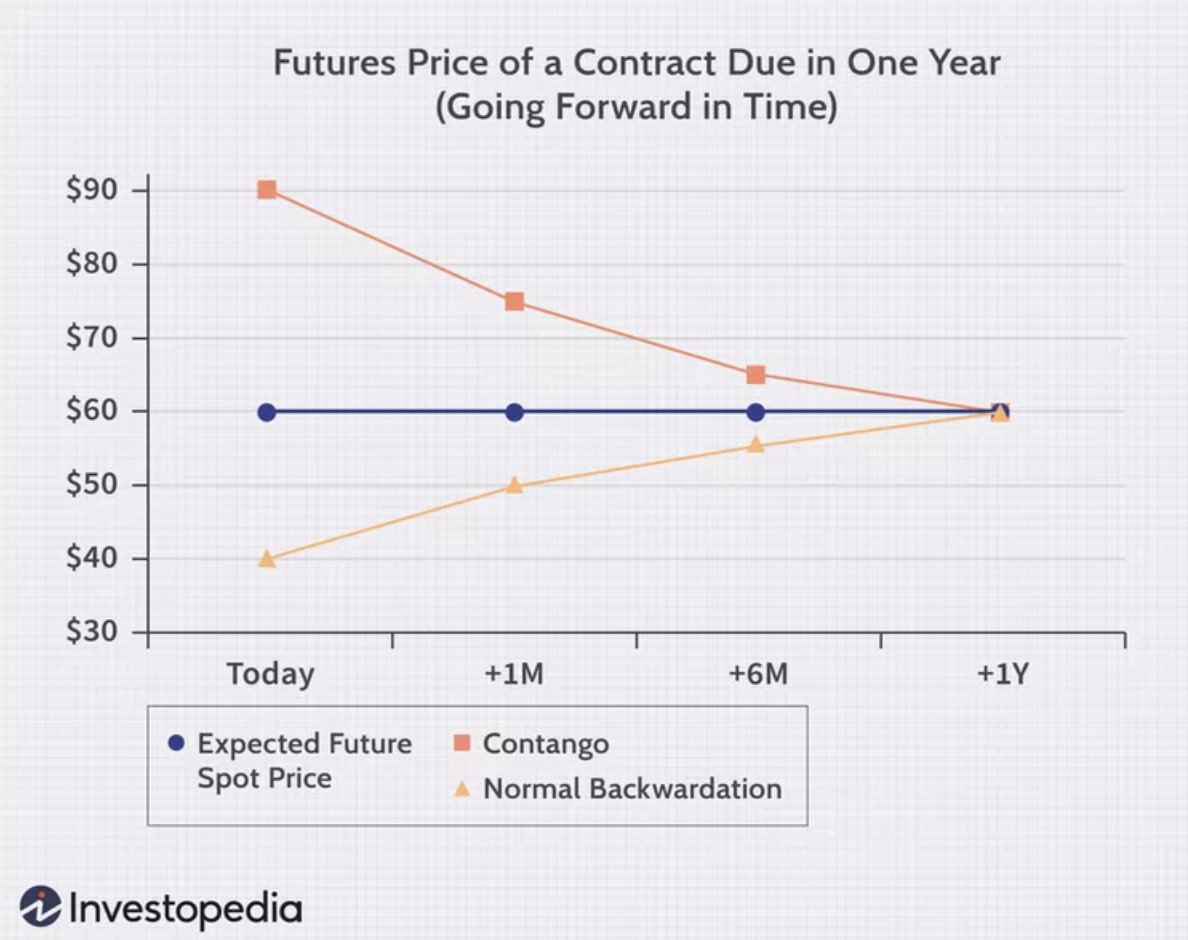
\includegraphics[width=0.8\linewidth]{futures_market.png}
    \caption{Futures Market (Source: Investopedia)}
    \label{fig:futures}
\end{figure}

\begin{enumerate}
    \renewcommand{\labelenumi}{\alph{enumi}.}
    
    \item Contango: \\ 
    Contango markets are often involving goods that don't have an immediate consumption date, i.e. precious metals. Contango can also be analogous to a normal curve; the idea is that consumers may be more willing to pay a higher price than the current spot price for a commodity in the future. Let's take the previous example of apples: The current spot price for apples are 20 cents/barrel, and the futures contract is priced at 50 cents per barrel. If a consumer buys at the spot price and stores until later to sell at the futures price, the current demand and current price for apples will increase. This implies that, in the future, people will be more likely to agree to sell, which will lower future prices.
    \item Normal Backwardation \\
    On the contrary, normal backwardation is based upon the theory that due to volatility, sellers are more inclined to sell at a lower price than the expected price in the future. 
\end{enumerate}

Backwardation is a indicator of a bullish market for the commodity, since it suggests the current value of the asset is the most valuable, which can be a sign of a shortage. Some severe contangos, on the other hand, can be an indicator of a bearish market, which can be caused by surplus or anticipated future shortage.

% \subsection{RMMs vs. AMMs}
\section{RMM \& CFMM Curves}
Since the goal of RMMs, as previously discussed, is to generate a trading function that models a specific trading fee payoff, we can represent the equation for an RMM given the CMM function. A CFMM is governed by its trading function \(\psi \) : \(\mathbb{R}^n_+ \to \mathbb{R}\).

Each reserve \( R_i \in \mathbb{R}^n_+ \) represents the amount of asset \(i\) available in the contract, which allows individuals to trade reserves as long as the following equation is satisfied: 
\[ \psi(R') \geq \psi(R), 
    \] with \(R \in \mathbb{R}^n_+\).

    For a non-decreasing, concave function
    \[V(\alpha c) = \alpha V(c), \alpha\in\mathbb{R}
        \]
    
    \(V\) is a portfolio value function which maps \(V: \mathbb{R}^n_+ \to \mathbb{R}\). We model asset \(c \in \mathbb{R}^n_+\) as a price vector representing \(n\) coins the CFMM trades, with \(c_i\) being the price of coin \(i\) in the external market. 

    The trading value is then defined with the following equation:
    \[
        \psi_V\left(R\right) = \inf_{c\geq0}(c^{\intercal}R - V\left(c\right)).\]
    
    Given this definition, it is shown that \(\psi_V\left(R\right)\) is defined as the greatest lower bound (infimum) of the expression \(c^{\intercal}R - V\left(c\right) \) over all non-negative vectors \(c\)

    Now, let's prove that \(\psi_V\left(R\right) \geq 0\) if and only if \(c^{\intercal}R \geq V(c) \forall c \in \mathbb{R}^n\), which is desirable since we want that the least surplus across all non-negative vectors \(c\) to be non-negative to ensure reserves \(R\) are always at least sufficient to meet required values \(V(c)\) under all possible weightings \(c\).

    Given \(\psi_V\left(R\right) \geq 0\), this implies the infimum (least upper bound) of all \(c^{\intercal}R - V\left(c\right)\) across all \(c \geq 0\) is non-negative, which implies that for every non-negative \(c\), the individual value \(c^{\intercal}R - V\left(c\right)\) is also non-negative. Therefore, \(c^TR-V(c) \geq 0 \implies c^TR \geq V(c)\). Since the infimum in this set is proven to be non-negative, this implies all values are at least as great.

    To prove the other direction, since for all \(c \geq 0, c^TR \geq V(c)\), each evaluation of \(c^TV(c)\) would yield a non-negative value. By the same logic, the greatest lower bound of all these values would also be non-negative. Therefore, the condition \(\psi_V\left(R\right) \geq 0\) is true if and only if \(R\) belongs to the set of reserves that yields a payoff greater or equal to \(V\).

% \section{Case Study: Primitive}
% Primitive's "RMM-01" is an example of a replicating market maker, built on the idea of a covered call.

% \begin{figure}[H]
%     \centering
%     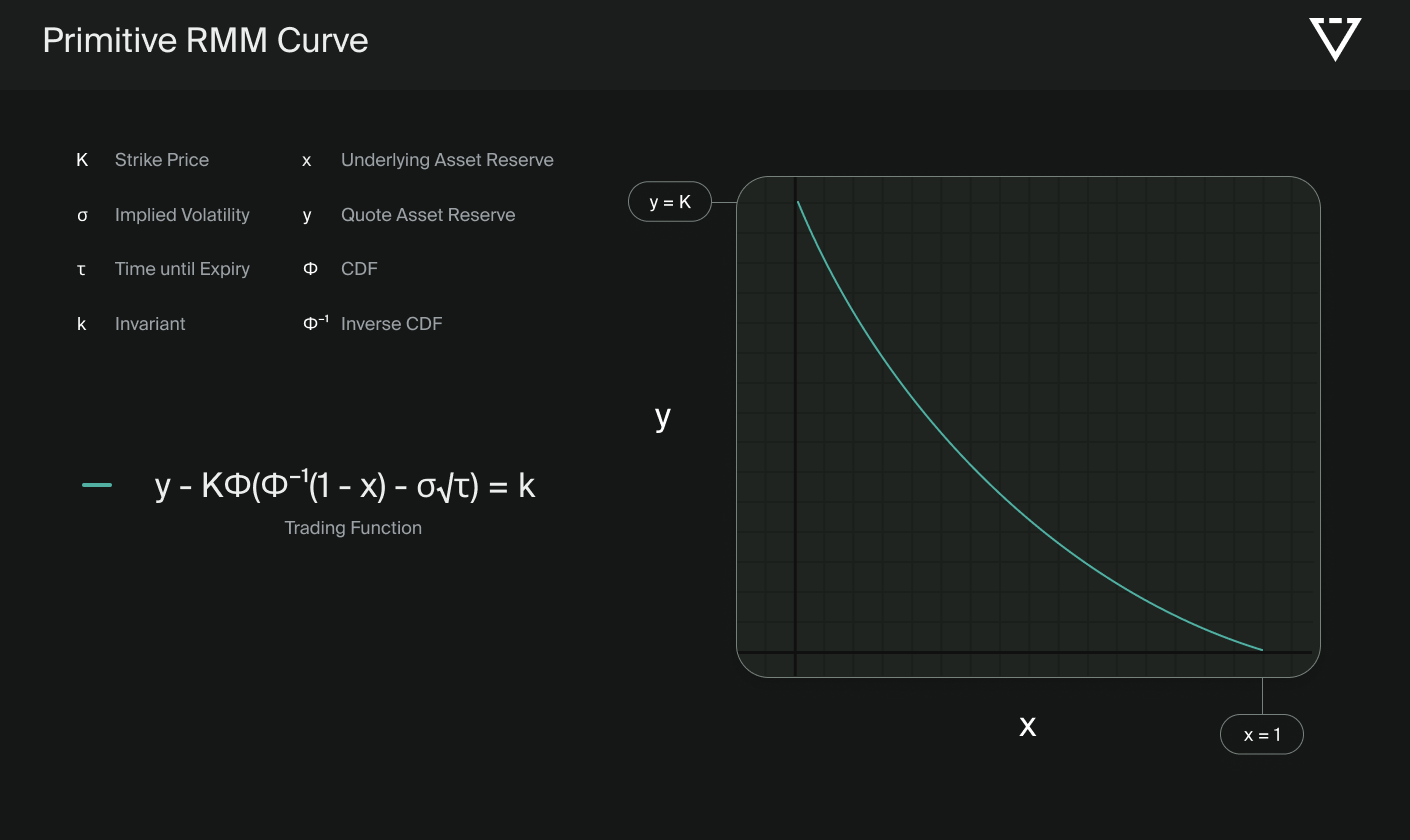
\includegraphics[width=0.8\linewidth]{Primitive.png}
%     \caption{Primitive's RMM Curve (Source: Primitive)}
%     \label{fig:primitive}
% \end{figure}


\section*{Appendix}

\subsection{Glossary}\label{subsec:glossary}
Infimum: The infimum, \(\inf\) of a set is defined to be the greatest lower bound of that set. More rigorously, we define \(\alpha\) to be the \(\inf\) of a set \(A\) if \(\forall x \in A, \alpha \leq x.\)
Furthermore, since \(\alpha\) is the greatest lower bound, if \(\beta \leq x, \forall x \in A\) and \(\beta \leq \alpha\), since \(\alpha\) serves as the greatest lower bound.

\subsection{Impermanent Loss}\label{subsec:impermanent}
\href{https://dailydefi.org/tools/impermanent-loss-calculator/}{Daily Defi} provides an impermanent loss calculator that can be used to visualize the calculations of impermanent loss using Uniswap's constant product formula.
In the following diagram, Token A is initially set to \$150 and Token B is set to \$1. In Future Prices, Token A has increased to \$300 while Token B has remained the same. (The calculator automatically sets a total starting value of \$1000 between the two tokens)
\begin{figure}[H]
    \centering
    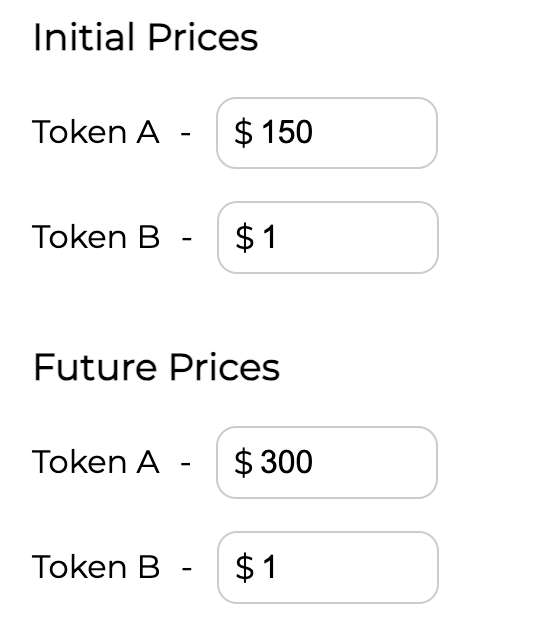
\includegraphics[width=0.4\linewidth]{impermanent_loss.png}
    \caption{Daily Defi's Impermanent Loss Calculator}
    \label{fig:impermanent_loss}
\end{figure}

Below, the results account for the total amount of impermanent loss. The value of Token A and B would be \$1500 if held, and \$1414.21 if provided as liquidity, thereby resulting in an impermanent loss of \$85.79.

\begin{figure}[H]
    \centering
    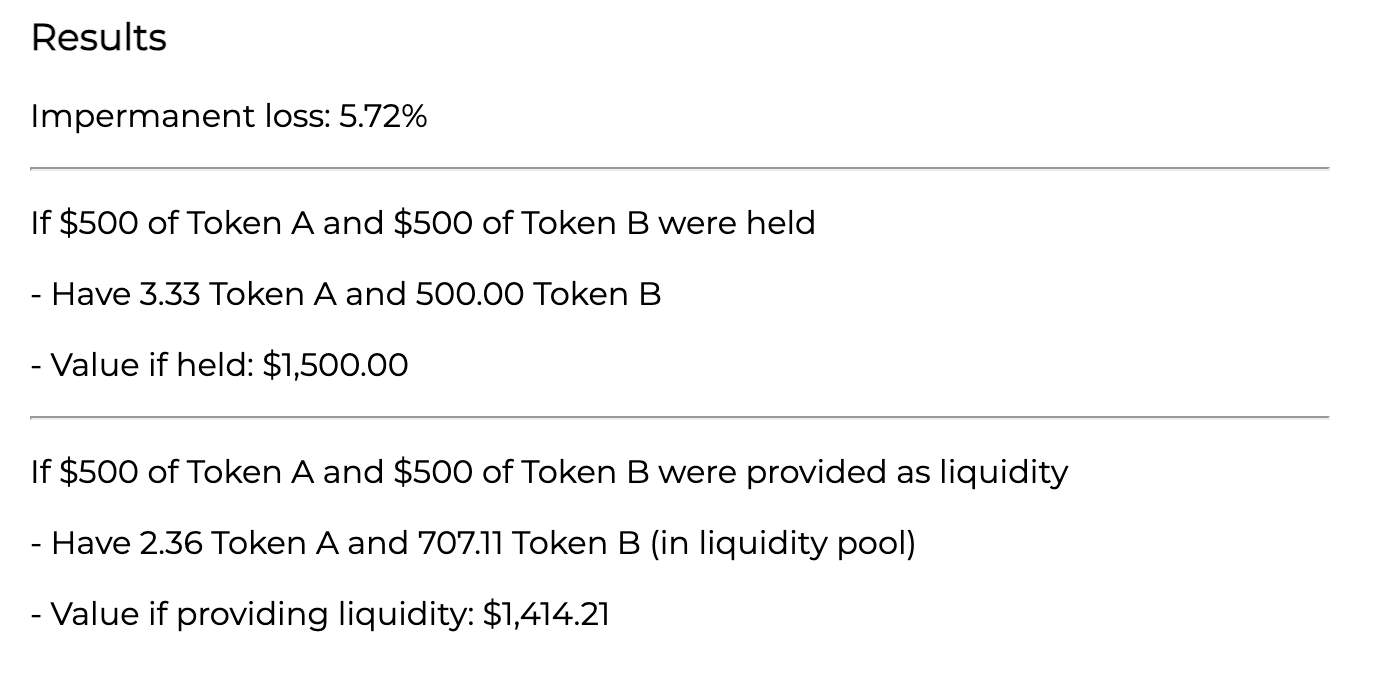
\includegraphics[width=0.6\linewidth]{results.png}
    \caption{Calculations of Impermanent Loss}
    \label{fig:calculations}
\end{figure}

\section*{References}
\begin{enumerate}
    \renewcommand{\labelenumi}{[\Alph{enumi}]}
    \item \href{https://medium.com/numoen/an-introduction-to-replicating-market-makers-de5c44d3c558}{An Introduction to Replicating Market Makers} (Numeon, 2021)
    \item \href{https://www.thetie.io/insights/research/rmm/}{Replicating Market Makers} (The Tie, 2021)
    \item \href{https://mirror.xyz/evandekim.eth/aUULTZFwhJ9XsOZ6XIbAYl1iaSncDKpDwKazCemJlI8}{Mirror.xyz: Replicating Market Makers by Evan De Kim} (2021)
    \item \href{https://chain.link/education-hub/what-is-an-automated-market-maker-amm}{What is an Automated Market Maker (AMM)?} (Chainlink Education Hub, 2021)
    \item \href{https://ui.adsabs.harvard.edu/abs/2021arXiv210314769A/abstract}{Automated Market Makers and the Universal Law of Demand} (Harvard ADS, 2021)
    \item \href{https://opynopyn.notion.site/Market-Makers-4ca991796d8b452fa1358344f941f624}{Market Makers} (Opyn Notion, 2021)
    \item \href{https://library.primitive.xyz/faq/usage/rmm}{Primitive.xyz RMM FAQ} (2021)
    \item \href{https://primitive.mirror.xyz/Audtl29HY_rnhN4E2LwnP7-zjDcDGAyXZ4h3QpDeajg}{Mirror.xyz: Primitive Finance RMM Explanation} (2021)
    \item \href{https://not-financial-advice.notion.site/RMMs-c5c6b0d9e190404c94d66241178454da}{RMMs Overview} (Not Financial Advice, 2021)
    \item \href{https://www.fidelity.com/learning-center/investment-products/options/call-options-basics}{Call Options Basics} (Fidelity Learning Center, 2021)
    \item \href{https://angeris.github.io/papers/rmms.pdf}{Replicating Market Makers: Theoretical Model} (Angeris et al., 2021)
    \item \href{https://web.stanford.edu/~boyd/papers/pdf/cfmm.pdf}{Constant Function Market Makers} (Stanford University, Boyd et al., 2021)
    \item \href{https://not-financial-advice.notion.site/Options-364981cc38bf4c55b45976a715d79604}{Options and Replicating Portfolios} (Not Financial Advice, 2021)
    \item \href{https://capital.com/replicating-portfolio-definition}{Replicating Portfolio Definition} (Capital.com, 2021)
\end{enumerate}

\end{document}


